%KECReportFormat.tex
%%%%%%%%%%%%%%%%%%%%%%%%%%%%%%%%%%%%%%%%%%%%%%%%%%%%%%%%%%%%%%%%%%%%%%%%%%%
%DO NOT MAKE CHANGES IN THIS FILE

\documentclass[12pt, a4paper]{report}
\usepackage[left = 1.5in, right = 1.25in, top = 1.25in, bottom = 1.25in]{geometry}%for margin
\usepackage{amsfonts, amsmath, amssymb} %for mathematical equations
\usepackage{graphicx} %for images
\usepackage{times} %font Times New Roman Font
\usepackage{float} %required if you use H(strictly here) position for floats
\usepackage[skip = 8pt,tableposition=top, figureposition=bottom]{caption}%adjust spacing of captions and specify where captions are
\usepackage{hyperref} % for easy Navigation in document, also puts links in TOC, LOF, LOT...
\usepackage{setspace} %to change line spacing in some portion \singlespacing \onehalfspacing \doublespacing
\usepackage{acro} %for List of Abbrreviation and Symbol
\acsetup{first-style = short} % set to display only short form on the command \ac{}

%packages required for complex tables
\usepackage{bigstrut} 
\usepackage{multirow}

\renewcommand{\contentsname}{Table of Contents} %Change TOC Heading ... default is "Contents" 

\parindent 0pt	%removes the indent in paragraph
\setlength{\parskip}{18pt}	%for paragraph spacing
\renewcommand{\baselinestretch}{1.5}   %Line Spacing = 1.5 line-spaces

%to reduce spacing in sections
\usepackage{titlesec}
\titlespacing*{\section}{0pt}{0pt}{0pt} %left, top, bottom spacings
\titlespacing*{\subsection}{0pt}{0pt}{0pt}
\titlespacing*{\subsubsection}{0pt}{0pt}{0pt}
\titlespacing*{\paragraph}{0pt}{0pt}{0pt}
\titlespacing*{\subparagraph}{0pt}{0pt}{0pt}

%adjust fontsizes\ of sections
\titleformat*{\section}{\fontsize{14pt}{18pt}\bfseries}
\titleformat*{\subsection}{\fontsize{13pt}{18pt}\bfseries}
\titleformat*{\subsubsection}{\fontsize{12pt}{18pt}\bfseries}
\titleformat*{\paragraph}{\fontsize{12pt}{18pt}\bfseries}
\titleformat*{\subparagraph}{\fontsize{12pt}{18pt}\bfseries}

%to reduce separation between points in list
\usepackage{enumitem}
\setlist[enumerate]{nosep} % no separation between items in enumerate
\setlist[itemize]{nosep} % no separation between items in itemize
%use \vspace{-18pt} before list to reduce paragraph spacing between list and preceeding paragraph.

%Changes for Chapter Heading Spacing and formats for numbered chapters
\makeatletter
\def\@makechapterhead#1{%
  %\vspace*{50pt}%
  {  \MakeUppercase{\ifnum \c@secnumdepth >\m@ne
        \fontsize{16pt}{1}\bfseries \@chapapp \space \thechapter\vspace{5pt}\\
    \fi
    \interlinepenalty\@M
     \bfseries #1}\par\nobreak
    %\vskip 0pt
  }}
\makeatother

%%%%%%%%%%%%%%%%%%%%%%%%%%%%%%%%%%%%%%%%%%%%%%%%%%%%%%%%%%%
%to adjust Heading spacings and fonts For unnumbered chapters, TOC, LOF ...
\makeatletter
% Redefine the \chapter* header macro to remove vertical space
\def\@makeschapterhead#1{%
  %\vspace*{50\p@}% Remove the vertical space
  {\newpage \parindent \z@ \raggedright
    \normalfont
    \interlinepenalty\@M
    \center \fontsize{16pt}{1} \bfseries \MakeUppercase{#1}\par\nobreak
    %\vskip 18\p@ % adjust space after heading 18pt
  }}
\makeatother 
%%%%%%%%%%%%%%%%%%%%%%%%%%%%%%%%%%%%%%%%%%%%%%%%%%%%%%%%%%%

%%%%%%%%%%%%%%%%%%%%%%%%%%%%%%%%%%%%%%%%%%%%%%%%%%%%%%%%%%%%%%%%%%%%%%%%%%%
% newcommand for generating Cover Page
\newcommand{\KECcoverpage}
{
\begin{titlepage}
\begin{center}
\Large{\textbf{KANTIPUR ENGINEERING COLLEGE}}\\
\large{\textbf{(Affiliated to Tribhuvan University)}}\\
\large{\textbf{Dhapakhel, Lalitpur}}\\
\vfill	%vertically fill the space 
\begin{figure}[h] % h: put logo "here"
\begin{center}

\includegraphics[width=25mm, height = 25mm]{images/logo.png}
\end{center}
\end{figure}

\large{\textbf{[Subject Code: \subCode]}}\\ %Change This Line
\large{\textbf{A \MakeUppercase{\project} \MakeUppercase{\doc} ON}}\\ %Change This Line
\Large{\textbf{\MakeUppercase{\projectTitle}}}\\

\vfill	%vertically fill the space 
\large{\textbf{Submitted by:}}\\
\large{\textbf{\submittedBy}}\\
\vfill	%vertically fill the space 
\textbf{A \MakeUppercase{\project} SUBMITTED IN PARTIAL FULFILLMENT OF THE REQUIREMENT FOR THE DEGREE OF \MakeUppercase{\degree}}\\

\vfill	%vertically fill the space 
\large{\textbf{Submitted to:}}\\
\large{\textbf{\submittedTo}}\\
\vfill
\large{\textbf{\defMonth, \defYear}}
\pagebreak
\end{center}
\end{titlepage}
}
%%%%%%%%%%%%%%%%%%%%%%%%%%%%%%%%%%%%%%%%%%%%%%%%%%%%%%%%%%%%%%%%%%%%%%%
% newcommand for generating Cover Page
%Title Page
\newcommand{\KECtitlepage}
{
\begin{titlepage}
\begin{center}
\Large{\textbf{\MakeUppercase{\projectTitle}}}\\

\vfill	%vertically fill the space 

\large{\textbf{Submitted by:}}\\
\large{\textbf{\submittedBy}}\\


\ifhassupervisor % Displays Supervisor name only if \hassupervisortrue
	\vfill	%vertically fill the space 
	\large{\textbf{Supervised by:}}\\
	\large{\textbf{\supervisor}}\\
	%\large{\textbf{\degSup}}\\
%	\large{\textbf{\orgSUP}}\\
\fi

\vfill	%vertically fill the space 
\textbf{A \MakeUppercase{\project} SUBMITTED IN PARTIAL FULFILLMENT OF THE REQUIREMENT FOR THE DEGREE OF \MakeUppercase{\degree}}\\

\vfill	%vertically fill the space 
\large{\textbf{Submitted to:}}\\
\large{\textbf{\submittedTo}}\\
\large{\textbf{Kantipur Engineering College}}\\
\large{\textbf{Dhapakhel, Lalitpur}}\\

\vfill
\large{\textbf{\defMonth, \defYear}}
\thispagestyle{empty}\\ %to remove page number
\pagebreak
\end{center}
\end{titlepage}
}
%%%%%%%%%%%%%%%%%%%%%%%%%%%%%%%%%%%%%%%%%%%%%%%%%%%%%%%%%%%%%%%%%%%%%%
%command for copyright page
\newcommand{\KECcopyright}
{
\chapter*{Copyright}%Required only for Final Defense of Major Project
\addcontentsline{toc}{chapter}{Copyright}
The author has agreed that the library, Kantipur Engineering Collage, may make this report freely available for inspection. Moreover the author has agreed that permission for extensive copying of this report for scholarly purpose may be granted by the supervisor(s), who supervised the project work recorded herein or, in their absence, by the Head of the Department wherein this project was done. It is understood that due recognition will be given to the author of this report and to the \submittedTo, Kantipur Engineering College in any use of the material of this report. Copying or publication or other use of this report for financial gain without approval of the \submittedTo, Kantipur Engineering College and author’s written permission is prohibited.\par Request for permission to copy or to make any other use of the material in this report in whole or in part should be addressed to:

Head\\
\submittedTo\\
Kantipur Engineering College\\
Dhapakhel, Lalitpur\\
Nepal
}
%%%%%%%%%%%%%%%%%%%%%%%%%%%%%%%%%%%%%%%%%%%%%%%%%%%%%%%%%%%%%%%%%%%%%%
%command for Approval Letter
\newcommand{\KECapproval}
{
\chapter*{Kantipur Engineering College
\vskip -10pt}%Required only for Final Defense of Major Project
\begin{center}
\fontsize{12.3pt}{1} %size decreaced to adjust department name in single line
\textbf{
\MakeUppercase{\submittedTo}\\ %for department name
}
\vskip 10pt
\fontsize{16pt}{1}
\textbf{APPROVAL LETTER}
\end{center}
\vskip -16pt
\addcontentsline{toc}{chapter}{Approval Letter}%
The undersigned certify that they have read and recommended to the Institute of Engineering for acceptance, a project report entitled \textbf{"\projectTitle "} submitted by \\
\submittedBy \\
in partial fulfillment for the degree of \degree. \par
{\vspace{25pt}
..........................................\\
Supervisor\\
\supervisor \\
\degSup\\
\orgSUP\\
\vspace{25pt}\\
..........................................\\
External Examiner\\
\external\\
\degExternal\\
\orgExt\\
\vspace{25pt}\\
..........................................\\
\hod\\
Associate Professor\\
Head of Department\\
\submittedTo
\vspace{10pt}\\
Date: \defMonth\space\defDay ,\space \defYear%
\singlespacing\par
} %single spacing for the texts inside {}
}

%command for list of abbreviations
\newcommand{\KECloa}
{
\chapter*{List of Abbreviations}
\addcontentsline{toc}{chapter}{List of Abbreviations}
\vskip -42pt % to reduce space due to invisivle acronym class name
{
\singlespacing
\printacronyms[include-classes=abbr, name= ]
}
}


%command for list of symbols
\newcommand{\KEClos}
{
\chapter*{List of Symbols}
\addcontentsline{toc}{chapter}{List of Symbols}
\vskip -42pt % to reduce space due to invisivle acronym class name{
{
\singlespacing
\printacronyms[include-classes=symbol, name= ]
}
}

%command to adjust toc, lof, lot spacing
\newcommand{\KECadjusttocspacings}
{
\parskip 0pt % to remove paragraph spacing in TOC, LOF ...
\renewcommand{\baselinestretch}{0.1} % to adjust line spacing in toc
\newcommand*{\noaddvspace}{\renewcommand*{\addvspace}[1]{}}
\addtocontents{lof}{\protect\noaddvspace} %remove extra vertical space in LOF
\addtocontents{lot}{\protect\noaddvspace} %remove extra vertical space in LOT
} %includes the file KecReportFormat.tex that include all necessary formattings
%%%%%%%%%%%%%%%%%%%%%%%%%%%%%%%%%%%%%%%%%%%%%%%%%%%%%%%%%%%%%%%%%%%%%%%%%%%
%Define Macros for Details of your Project
\newcommand{\project}{Major Project} %Specify "Major Project" or "Minor Project"
\newcommand{\projectTitle}{"PROJECT X : A BUSINESS INTELLIGENCE FOR BIKE INSURANCE"} %specify "Title" of Your Project
\newcommand{\doc}{Pre-Final Report} % specify the document you are preparing eg. "Proposal", "Mid-Term Report" or "Final Report" 
% Note that You have to sibmit "Final Report" for Pre-final defense as well.
\newcommand{\subCode}{CT755} %specify Subject of Your Project
\newcommand{\degree}{Bachelor in Computer Engineering} %specify your degree
\newcommand{\submittedBy}%Specify Names and Roll/Symbol Numbers of the Project Group Members
{
%Edit Member Names and Roll/Symbol No. and adjust width (\makebox[width]) if necessary 
\makebox[9cm]{Amit Dhoju \hfill [091/BCT/2071]}\\
\makebox[9cm]{Kaushtup Bista \hfill [103/BCT/2071]}\\
\makebox[9cm]{Roshi Maharajan \hfill [117/BCT/2071]}
%\makebox[9cm]{Member Name \hfill [Roll/Symbol No.]}\\
} % Note that You must write your "Symbol Numbers"(Exam Roll Numbers) for Final Defenses

\newcommand{\submittedTo}{Department of Computer and Electronics Engineering} %specify your department
\newcommand{\hod}{Er. Rabindra Khati} %specify Head ot the department
\newcommand{\defYear}{2018} %Defense Year
\newcommand{\defMonth}{August} %Defense Month- January, February, ...
\newcommand{\defDay}{12} %specify Defense Day- 1, 2, ...

\newif
\ifhassupervisor
\hassupervisorfalse % to display supervisor name use command- \hassupervisortrue
 
\newcommand{\supervisor}{Ajay Mani Paudel} % Specify Name of Supervisor for Major Project
\newcommand{\degSup}{External Director} %Specify Designation of Supervisor for Major Project, use multiple lines (\\) if necessary
\newcommand{\external}{External's Name} %Specify Name of External for Major Project (Required for Black Book)
\newcommand{\degExternal}{External's Designation\\Second Line of Designation (if required)} %Specify Name of External for Major Project (Required for Black Book) , use multiple lines (\\) if necessary


%%%%%%%%%%%%%%%%%%%%%%%%%%%%%%%%%%%%%%%%%%%%%%%%%%%%%%%%%%%%%%%%%%%%%%%%%%%

%%%%%%%%%%%%%%%%%%%%%%%%%%%%%%%%%%%%%%%%%%%%%%%%%%%%%%%%%%%%%%%%%%%%%%%%%%%
%Define Abberviations and Symbols
% NOTE that Only those Abberviations and Symbols that are included in document(using command \ac{}) will be displayed in the List of Abberviations and Symbols.

%class 'abbr': for List of Abbreviations
\DeclareAcronym{bi}{ 
  short = BI ,
  long  = Business Intelligence ,
  class = abbr
}% declares acronym named "UN". Use \ac{UN} for short and \acl{UN} for long form. 

\DeclareAcronym{cc}{
  short = CC ,
  long  =  Cubic Centimeter,
  class = abbr
}

\DeclareAcronym{sdlc}{
  short =  SDLC,
  long  =  Software Development life Cycle,
  class = abbr
}
\DeclareAcronym{sql}{
  short =  SQL,
  long  =  Server Query Language,
  class = abbr
}

\DeclareAcronym{mvc}{
  short =  MVC,
  long  =  Model View Controller,
  class = abbr
}

\DeclareAcronym{nn}{
  short =  NN,
  long  =  Neural Network,
  class = abbr
}

\DeclareAcronym{svm}{
  short =  SVM,
  long  =  Support Vector Machine,
  class = abbr
}
\DeclareAcronym{csv}{
  short =  CSV,
  long  =  Comma Seprated Value,
  class = abbr
}
\DeclareAcronym{odbc}{
 short = ODBC,
 long =Open Database Connectivity,
 class = abbr
}
\DeclareAcronym{os}{
 short = OS,
 long =Operating System,
 class = abbr
}



%The Document
\begin{document}

\KECcoverpage % command defined in KECReportFormat
\KECtitlepage % command defined in KECReportFormat

\pagenumbering{roman} % starts pagenumberins in Roman numerals i, ii, ...

%Copyright Page is required for FINAL REPORT only. Comment this section for other Reports.
%\KECcopyright % defined in KECReportFormat.tex

%Approval Page is required for FINAL(Black Book Binded) REPORT of MAJOR PROJECT only. Comment this section for other Reports. 
%\KECapproval % defined in KECReportFormat.tex

\chapter*{Abstract} % The summary of your report
\addcontentsline{toc}{chapter}{Abstract}%to include this chapter in TOC 
 
There is no alternative for intelligence. What if intelligence used in gambling? the result is success. In short this is our project, title "\textbf{Project X:A Business Intelligence For Bike Insurance}". Our project describe a predict policy for bike insurance by visualization towards the history of bike insurance data. Our system will train for our intelligence and will be able to predict the possible claim. The insurance industry worldwide is facing the challenges of deregulation, consolidation and convergence of financial services. There is today a pressing demand for cutting edge services of insurance business management and enriched customer experiences at a significantly lower cost. Insurance is gambling and we are trying to give technique to win this gamble. Our system will determine the possible accident of bike so that management of insurance in-charge policy for new client whether to insurance or not. If system predicts the possible claim then system will suggest the insurance company not to make that insurance otherwise insurance is made. Based upon \acs{cc} of Bike, Bike Manufacturer, Lote, Zone, and Type Cover, our system will predict the possible claim.
\par
\textbf{\textit{Keywords$-$}} Business Intelligence, Prediction, Analysis, Insurance 

%\chapter*{Acknowledgment}
%\addcontentsline{toc}{chapter}{Acknowledgment}%to include this chapter in TOC
%Write Acknowledgment Here. Ea his munere torquatos, quidam essent luptatum cu pro. Ei duo scaevola %electram. Vidit percipitur ut vim, ne his solet prodesset inciderint. Cum facilisi sententiae at, vis %noster electram contentiones cu. Nec at eius novum diceret.
%\par
%%Second para of Acknowledgment. Sed veri aeque persecuti ut. Ut accusam mediocrem accusamus eos, quis %clita probatus ex his. Mea oratio deleniti interesset at. Odio melius antiopam eu his, ut nec tantas maiestatis ullamcorper. Ut numquam reprimique cum. Acknowledgement ENDS here.\par

%{to display members name under Acknowledgement
\begin{flushright}
\vskip -20pt
\setstretch{1.2}
\submittedBy
\end{flushright}
%
%to adjust spacings for TOC, LOF, LOT
{
%%%%%%%%%%%%%%%%%%%%%%%%%%%%%%%%%%%%%%%%%%%%%%%%%%%%%%%%%%%%%%%%%%%%%%%%%%%
%TOC, LOF and LOT
\KECadjusttocspacings % defined in KECReportFormat.tex to adjust spacings
\makeatletter
% to add vskip of 18 point which is reduced when parskip is set to 0 in \LECadjustspacings
\def\@makeschapterhead#1{%
  %\vspace*{50\p@}% Remove the vertical space
  {\newpage \parindent \z@ \raggedright
    \normalfont
    \interlinepenalty\@M
    \center \fontsize{16pt}{1} \bfseries \MakeUppercase{#1}\par\nobreak
    \vskip 18\p@ % adjust space after heading 18pt
  }}
\makeatother 

\tableofcontents % prints table of contents

\cleardoublepage
% \phantomsection
\addcontentsline{toc}{chapter}{\listfigurename}
\listoffigures
%\listoffigures % prints list of figures
%\listoftables % prints list of table
}
%%%%%%%%%%%%%%%%%%%%%%%%%%%%%%%%%%%%%%%%%%%%%%%%%%%%%%%%%%%%%%%%%%%%%%%%%%%

%comment this chapter if you don't have List of Abbreviations
\KECloa % defined in KECReportFormat

%comment this chapter if you don't have List of Symbols
%\KEClos % defined in KECReportFormat

\newpage
\pagenumbering{arabic} % starts pagenumbering in arabic numerals

\chapter{Introduction}

\section{Background}\label{sec:bkgrnd}%label your section if you require to refer them somewhere else in \textbf{your document.
\textbf {\acl{bi}}(BI) is defined as the ability for an organization to take all its capabilities and convert them into knowledge. This produces large amounts of information which can lead to the development of new opportunities for the organization. When these opportunities have been identified and a strategy has been effectively implemented, they can provide an organization with a competitive advantage in the market, and stability in the long run.\cite{chen2012business}
\par
Business Intelligence in Insurance provides the information to insurance company on claim management of motorbike which helps in gain insight and visibility on the cost of claims; analyze claims breakdown by \acs{cc} of Bike, Bike Manufacturer, Lote , Zone and Type Cover. 
To predict and analyze the insurance historical data based on the claims, data can identify suitable polices for risk modelling , reinsurance, profitability analysis, loss analysis, claim analysis, claim estimation by  using the “ Back propagation algorithm ” to find the claim pattern according to \acs{cc} of Bike, Bike Manufacturer, Lote, Zone, and Type Cover.
Some insurers have gone for non-scalable temporary solutions, which often fail to leverage the ever-increasing volumes of data. Hence, recognizing the need for an effective business a data warehouse cannot be the answer to all the information requirements hence it is also very important to set clear business objectives for the business intelligence solution with total top management support.
 \par
\newpage
\section{Insurance}
A practice by which a company provides a guarantee of compensation for specified loss, damage, illness, or death in return for payment. 
\subsection{Definition of Non-Life Insurance }
Non-life insurance, also called property and casualty insurance, is a type of coverage that is very common and covers businesses and individuals. It protects them, monetarily, from disaster by providing money in the event of a financial loss. Before you purchase this type of insurance or if you already own any kind of non-life insurance, you should understand what it is.

\subsection{Principle of Insurance}
\begin{enumerate}
\item Insurance transfers the financial consequences of an existing risk.
\item Law of Large Numbers
\item The more predictable the outcome
\item Pricing and risk management
\item Considerations in Setting Premium Rates
\end{enumerate}

\newpage
\subsection{Insurance Risk}
\begin{itemize}
	\item Some examples of insurance risk:
	\begin{enumerate}
		\item Legal - litigation
		\item Operational - mistakes, errors, etc.
		\item Pricing - inadequate premiums
        \item Regulatory - new requirements
        \item Reputation - negative press
	\end{enumerate}
\end{itemize}
A schematic overview over the different quantitative risk factors for non-life insurance can be given as:
\begin{figure}[tbh] % tbh means top, bottom or here (priority: left to right)
\begin{center}
	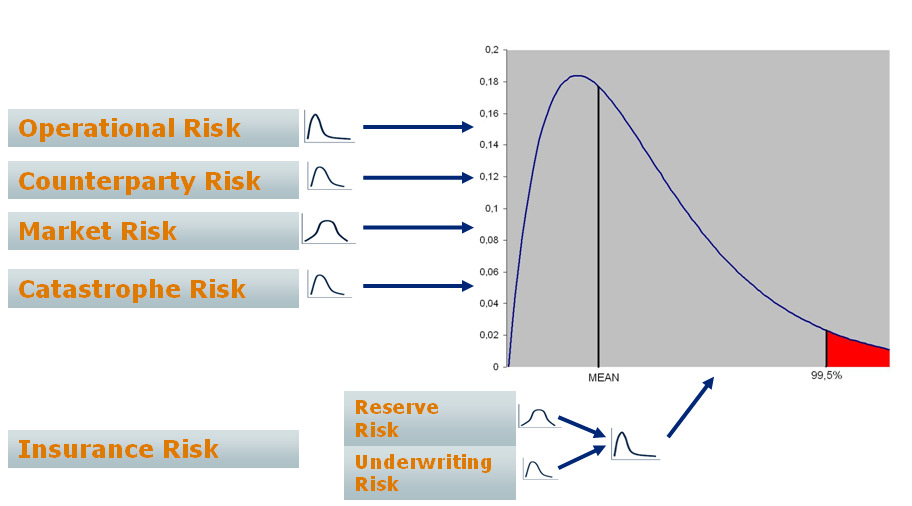
\includegraphics[width = 5in]{images/ir.png}
	\caption{Insurance Risk}\cite{grevskott_2011} %figure name


	\label{Risk type}% for referencing
\end{center}
\end{figure}
\par
Some of the type non-life insurance arelisted below:\cite{grevskott_2011}
\begin{enumerate}


\item \textbf{Operational Risk}
\par
Operational risk is usually considered as risks connected to the people, systems and processes in a business. This is a very broad group of risk and includes fraud, system failures, terrorism and employee compensation claims. The model for operational risk may be very complex with detailed models for each element influencing the risk, but simplified models based on some appropriate exposure figure is also common. For non-life insurance a factor of earned premium is commonly used.
\par
\item \textbf{Counter-party Risk}
\par
The risk of not receiving payment as agreed is often called counterparty or credit risk and the event is often called default. For non-life insurance the counterparty is often a reinsurer. The probability of default (PD) is often given by credit rating agencies like S\&S  and Moody’s. The value at risk is simply the amount at stake multiplied by the probability of default given by the rating agencies. An example of rating and default probabilities are: A further sophistication of this model is to give a distribution of the loss given default.
\par
\item \textbf{Market Risk}
\par
When modelling market risk we want to find how much the company assets may decrease due to change in the market factors. The four standard market risk factors are stock prices, interest rates, foreign exchange rates, and commodity prices. The actual portfolio of the company decides which factors are to be taken into consideration. Usually one wants to model these factors as time series and a lot of work is done in this field. However, most insurance companies will rely on Economic Scenario Generators (ESG) as a part of a risk management tool rather than develop own methods for market risk.


\item \textbf{Insurance Risk}
\par
Insurance risk is the risk arising from the process of transferring risk from persons or companies to the insurance company and it is the fundamental business idea of an insurance company. It is usually divided in two main categories: underwriting risk and reserve risk. Underwriting risk is the risk arising from claims incurring in future accounting periods, while reserve risk is the risk arising from previous accounting periods.

\item \textbf{Underwriting Risk}
\par
To be able to predict the claims for a future accounting period we need to know about the claims in previous accounting periods. We will show an example on how to model next periods claims based on historical claims. To give an example we have accumulated periodical claims data from two lines of business, health insurance and workman’s compensation insurance.

\end{enumerate}

\section{Crystal Report}
Crystal Reports is a popular Windows-based report writer (report generation program) that allows a programmer to create reports from a variety of data sources with a minimum of written code. Developed by Seagate Software, Crystal Reports can access data from most widely-used databases and can integrate data from multiple databases within one report using \acl{odbc} (\acs{odbc}). Crystal Reports uses an ActiveX control called Crystal Report to establish a connection with another program. A programmer can set properties of the Crystal Report control during design time or at run time.
\par
The programmer can use automation tools called Experts to be guided through common tasks, such as linking and embedding reports. Crystal Reports treats all text, graphics, and database fields as object s that a programmer can place, arrange, and format on forms. The program also generates a record set object and code needed to perform programming tasks such as loop s or mathematical calculations. Crystal Reports can create a report on the fly from user-defined variables and can convert it to HTML and publish it to the Web automatically. 

\section{Problem Statement}
The insurance industry worldwide is facing the challenges of deregulation, consolidation and convergence of financial services. There is today a pressing demand for cutting edge services of insurance business management and enriched customer experiences at a significantly lower cost. Our project aims to predict the risk behind bike insurance. It relates the information of the current customer and bike to the past data determining whether to make insurance or not.

\newpage
\section{Objectives}\label{sec:obj}
The objectives of this project are:
\begin{itemize}
\item \textbf{To predict the possibility to claim of bike insurance}
\par 
\par We have created a classifier model with inputs CC of Bike, Bike Manufacturer, Lote, Zone, and Type Cover. And the claim status is given to determine the claim of the insurance. Hence, our system with the above mentioned parameter will be able to predict the possible claim.
\item \textbf{To visualize the insurance performance} 
\par 
We have used bar chart to visualize the claim and un-claim data for each individual attributes. This visualization will show total insurance of particular field of particular attributes, claim count of that attribute un-claim count of that attribute. Hence our system visualize the overall performance of the insurance
\item \textbf{To generate the claimed and unclaimed report}
Report is another objective of our system. Our system allows user to select the particular attribute, then total claimed and unclaimed data count of particular field of an attribute is displayed simultaneously. This will report to the management level for the decision for overall performance of the insurance. System is able to print the report.
\end{itemize}

\section{Application}
Project-X is a web application which analyze and visualize the user data. This project is specally developed for insurance company. The application of this is help the  management level for policy making in insurance company. It provides visualization to the company. The visualization generate the report for claimed and unclaimed report separately with respective attributes. The report provides the management level with overall glance of the insurance to claim policy. The generated report is printable. Due to this , it required less human resource. In simple meaning it is decision support system for bike insurance company.

\section{Project Features} \label{sec:feat}
\begin{itemize}
\item Claimed and unclaimed report generation based on various attributes.
\item Insurance performance can be visualized. 
\item Business Intelligence Report (Crystal Report). 
\end{itemize}






\section{Feasibility Analysis}

\subsection{Economic Feasibility}

The economic feasibility of the software refers to the cost of its creation, cost required
to launch the system and its efficiency in terms of cost after its launch to real platform.
It determine whether the project is economically and logically possible or not.  This
project reduces the operations and maintenance cost of IT infrastructures

\subsection{Technical Feasibility}
This feasibility includes the software and hardware used for project.As this project will be developed using 'C sharp' as programming language and simply using the logical concept, it won't require sophisticated equipment. A PC with any Operating System with a browser and network will be able to run the software. Almost all current devices support the surfing the network. Thus watching overall ,this project is technically feasible.

\subsection{Operational Feasibility}
A feasibility study aims to objectively and rationally uncover the strengths and weaknesses of a project. As a webpage, it can be anywhere at any time after it deployment to the server. Our project provides user friendly platform, people with simple knowledge of computer can operate easily and the system can perform the rest operation.

\newpage
\section{System Requirement}
System Requirements are categorized  into two field:
\subsection{Software Requirement}
\begin{itemize}

\item{}\textbf{For System Development}
 \begin{enumerate}
 \item Operating System : Windows \acs{os}
 \item IDE : Visual Studio 2017
 \item Framework : Microsoft .net framework
 \item Database : Microsoft SQL Server 2014
 \end{enumerate}

\item \textbf{For End Users} 
\begin{enumerate}
\item Any Operating System with browser and internet.
\end{enumerate}

\end{itemize}

\subsection{Hardware Requirement}
\begin{itemize}
\item \textbf{For System  Development}
\begin{enumerate}
\item PC with 1.8 GHz 4 GB RAM
\end{enumerate}
\item \textbf{For End Users}
\begin{enumerate}
\item Any Device with supporting latest browser and internet
\end{enumerate}
\end{itemize}


\chapter{Literature Review}
Insurance is a practice by which a company provides a guarantee of compensation for specified loss, damage, illness, or death in return for payment.Bike Insurance is insurance for bike, motorcycle. Its primary use is to provide financial protection against physical damage or bodily injury resulting from traffic collisions and against liability that could also arise there from. Bike Insurance also provide financial support in case of bike stolen, damaged to bike from events other than traffic collisions , and keying and collision with stationary object. \cite{insurance2015bike}
Some Previously developed platform:
\par
\section{Sisense}
 \par
Sisense is \acl{bi} software by Sisense Inc.,the  industry in for complex data-easily prepare analyze and explore growing  data from multiple sources. Sisense is awarded with \textbf{Best \acl{bi} Software for    2016}. It is the business analytics software that lets you easily
prepare and analyze big, scattered datasets. it have 3 types of user 
\begin{enumerate}
\item[i.] Admin : Can access all features of Application.
\item[ii.] Designer : Mainly to design the elastic cubes and all admin function except Serve and user management.
\item[iii.] Viewer : Can only view data result and visualization.
\end{enumerate}
\par The  unique about Sisense are :

\begin{enumerate}
\item[1.] Single-Stack architecture: A single tool that helps you collect, prepare, organize and analyze data.
\item[2.] In-chip Engine and Proprietary technology.
\item[3.] Optimal use of computational resources.
\item[4.] A 90-minutes real test-drive for prospective client.
\end{enumerate}
\par
\subsection{How Sisense work}
Sisense is webapp that work on  both Computer or in smartphones. It works on the dashboard system with Elastic Cubes which is the proprietary analytical tools database that enables to connect multiple data sources and run complex queries in split of second. The data sources that can be used with sisense are file-based data sources (Excel ,\acs{csv}), Traditional database (\acs{sql}, MySQL, Oracle) and Online Web-Services(Google adwords). Data sources are added in elastic cube manager.
 Different  types of data sources can be added in same cube. Any two field with same type of data on different data sources and be connected by drag and  drop facility of sisense. At last, by building elastic cubes the data will be pull form data sources into elastic cube. When the result is ready it is ready for calculation and the result can be visualize in multiple form.
\newpage

\section{Qlik Sense}
QlikSense is software launch  by Qlik software company. QlikSense lets you discover insights that query-based \ac{bi} tools simply miss. One can freely search and explore across  all his data, instantly pivoting your analysis when new ideas surface.\cite{troyansky2015qlikview}
\linebreak
The  unique about QlikSense are :

\begin{enumerate}
\item[1.] Full spectrum of visual analytic.
\item[2.] Externally governed assets and data modules.
\item[3.] Data compression.
\item[4.] Policy-based security rules
\end{enumerate}
\par
\subsection{How does Qlik sense work}
Qlik Sense is platform of data analysis. It analyze data and make discovery on your own.One can easily share knowledge and data in organization using Qlik sense. It generates views on information for the user. It does not require predefined and static reports. One do not have to dependent on other resources just click and learn. Each click sends instant responds updating every visualizations and view in the app with new data and visualizations. App model help by asking question and user can answer the next question on their own without going back to expert for new report or visualizations for the data .
\chapter{Theory}
\section{Bayes' Theorem}
\par
Bayes’ Theorem is a statement from probability theory that allows for the calculation of  certain conditional  probabilities. Conditional  probabilities  are  those  probabilities  that reflect  the influence  of  one  event  on  the  probability  of  another  event. The  term  generally used in Bayes’ theorem are prior probability and posterior probability. The prior probability of a hypothesis or events the original probability obtained before any additional information is obtained. The posterior probability is the revised probability of the hypothesis using some additional information or evidence obtained.\cite{garg2013design}
\par Bayes’ Theorem can be written as:

\[P(A|B)=\frac{P(B|A)P(A)}{P(B)}\]

Where,
\begin{enumerate}
\item P(A) is the prior probability of A , 
\item P(B) is the prior probability of B ,
\item $P(A | B)$ is the posterior probability of A given B \&
\item $P(B | A)$ is the posterior probability of B given A
\end{enumerate}

\par 
Bayes' Theorem for n independent variable:
\textbf{\[P(B|A)=P(B_1|A)*P(B_2|A)*P(B_3|A)*...*P(B_n|A)\]}

\section{Classification}
\par
Classification in data analysis is the task of assigning a class to instances of data described by a set of attributes. Classification or supervised classification includes the construction of a classifier which is trained on a set of training data
that already has the correct class assigned to each data point. This builds a concise model of the distribution of 
class labels. It is then used to classify new data where the values of features are known but the class is unknown.
\par
Many algorithms have been developed for supervised classification based on
\begin{itemize}
	\item[1.] Artificial Intelligence
	\item[2.] Perceptron-based Techniques (Single and Multi-Layered Perceptron)
	\item[3.] Statistical Learning Techniques (Bayesian networks,Instance based techniques)
\end{itemize}


\section{Bayesian Classification}
\par
Bayesian Network provides a powerful graphical method for encoding the probabilistic relationship among a set of variables and hence and naturally be used for classification. It learned by using likelihood to achieve classification accuracy. It learned by supervisied learning, where a  training data set of instances with labels representing instance of classes is used to train as classifier.\cite{garg2013design}
\linebreak Likelihood is calculated by:

\[CLL (G|D)=\sum_{i=1}^{N}\log P(C_i|V_i) \]
\newpage
\par
\subsection{Learning Models}
\par 
Types of Learning models:
\begin{enumerate}
\item[1.] \textbf{Generative Model}
\par
Generative models summarize data probabilistically and are more flexible,since the user can bring in conditional independence assumptions, priors, and hidden variables. Generative classifiers learn a model of the joint probability of the variables and the related class label, and use Bayes’ theorem to compute the posterior probability of the class variable and make predictions. 

\item[2.] \textbf{Discrimative Model}
\par
Discriminative models (e.g.\acs{nn} and \acs{svm}) only learn from data to make accurate predictions by directly estimating the class posterior probability or via discriminant functions, and thus offer the user less flexibility in data representation and inference.
\item[.] 
\end{enumerate}
\section{Na\"{\i}ve Bayesian Classifier}

\par
A Na\"{\i}ve Bayes Classifier is a probabilistic classifier based on applying Bayes’ theorem with strong independence  assumptions. When represented as a Bayesian network, a Na\"{\i}ve Bayes classifier has the structure depicted in Figure below.  \cite{friedman1997bayesian} It shows the independence assumption among all features in a data instance.
\begin{figure}[bh] % tbh means top, bottom or here (priority: left to right)
\begin{small}

	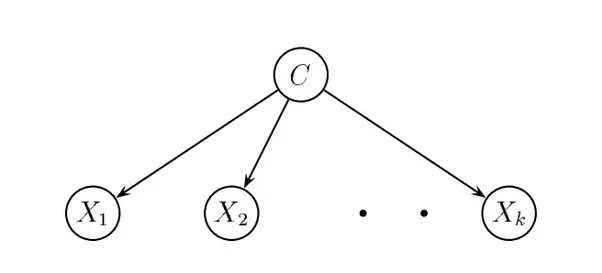
\includegraphics[width=4in]{images/naivebayesian.jpg}
	\caption{Structure of Na\"{\i}ve Bayesian Network} %figure name
	\caption*{Source:   http://www.mdpi.com/1099-4300/19/6/247}
	\label{NB} % for referencing
\end{small}
\end{figure}

\par
Na\"{\i}ve Bayes Classifier is simple probabilistic classifier that calculates a set of probability by counting the frequency and combinations of value in a given set of data. The algorithm uses Bayes theorem and assumes all attributes to be independent given the value  of  the  class  variable. Na\"{\i}ve Bayesian classifier is based on Bayes’ theorem and the theorem of total probability. 


\section{Data Pre-Processing}\label{sec:obj}
\begin{itemize}
\item Pre-process Steps
	\begin{itemize}
	\item[-] Data Cleaning
	\item[-] Data Integration and Transformation
	\item[-] Data Reduction
	\end{itemize}
\item Data in real world is dirty 
	\begin{itemize}
	\item[-]incomplete: lacking attribute values, lacking certain attributes of interest, or containing only aggregate data
	\item[-] noisy: containing errors or outliers
	\item[-] inconsistent: containing discrepancies in codes or names
    
	\end{itemize}
\item No quality data, no quality mining result
	\begin{itemize}
	\item[-] Quality decisions must be based on quality data
	\item[-] Data warehouse needs consistent integration of quality data
	\item[-] Reduced Accuracy
	\end{itemize}
\end{itemize}     
    
    
    
\subsection{Measure of data Quality}
    \begin{itemize}
    \item[•] \textbf{Well-accepted multidimensional view:}
    \begin{itemize}
    \item[-] Accuracy
    \item[-] Completeness
    \item[-] Consistency
    \item[-] Reliable
    \item[-] Interpretability         
    \item[-] Accessibility
    \end{itemize}     
    \end{itemize}

\subsection{Major Task in Data Pre-processing}    
\begin{enumerate}
\item Data Cleaning
	\begin{itemize}
	\item Fill in missing values, smooth noisy data, identify or remove outliers, and resolve 		inconsistencies.
	\item Data cleaning tasks
		\begin{itemize} 	
		\item Fill in missing values
		\item Identify outliers and smooth out noisy data 
		\item Correct inconsistent data	
		\end{itemize}
	\end{itemize}
 	
\item Data integration	
	\begin{itemize}
	\item Combine data from multiple data source.
	\item Detecting and resolving data value conflicts
	\item possible reasons: different representations, different name
	\end{itemize}
   
\item Data Transformation
	\begin{itemize}
	\item Normalization and aggregation
	\item Data smoothing
	\item Data summarization
	\item Data Reduction
	\end{itemize}
\end{enumerate}


\subsection{Data Smoothing}
When data collected over time displays random variation, smoothing techniques can be used to reduce or cancel the effect of these variations. When properly applied, these techniques smooth out the random variation in the time series data to reveal underlying trends. The variation  in data cause the program to  produce unreliable result and inaccurate. Smoothing is technique to remove the variation in data. 
\par
Different ways of data smoothing technique are:
\begin{enumerate}
%\renewcommand{\labelenumi}{\roman*.}
\item \textbf{Data Level approach: Resampling Techniques}
	\begin{enumerate}
	\item Random Under-Sampling
	\item Random Over-Sampling
	\item Cluster-Based Over Sampling
	\item Informed Over Sampling:Synthetic Minority Over Sampling Technique (SMOTE)
	\item Modified synthetic oversampling technique(MSMOTE)
	\end{enumerate}

\item \textbf{Algorithmic Ensemble Techniques}
	\begin{enumerate}
	\item Bagging based
	\item Boosting Based
		\begin{itemize}
		\item[-] Adaptive Boosting-Ada Boost
		\item[-] Gradient Tree Boosting
		\item[-] XG Boost
		\end{itemize}
	\end{enumerate}

\end{enumerate}
\subsection{SOMTE Technique}
\textbf{SMOTE} is short hand for Synthetic Minority Over Sampling Technique. This techniques is followed to avoid overfitting which occurs when exact replicas of minority instances are added to the main dataset. A subset of data taken from a minority class as an example and then synthetic similar instances are created. The synthetic instances are then added to the original dataset. Then the new data set is used to train the classifier models.\cite{witten2016data}
\par 
We have seperately perform data smoothing using R languages. We used SMOTE to balance the data of claimed and unclaimed data to maintain low variation and train the balanced data using Gradient boosting algorithm in R. 
\par 
This process significantly impacts the accuracy of the predictive model.  By increasing its around accuracy by 20 \%.

\section{Confusion Matrix}
A confusion matrix is a table that is often used to describe the performance of a classification model (or "classifier") on a set of test data for which the true values are known. The confusion matrix itself is relatively simple to understand, but the related terminology can be confusing.	
\par 
Confusion matrix is 2x2 matrix with 4 variables with Actual true and false and Predicated true and false class .

\begin{figure}[tbh] % tbh means top, bottom or here (priority: left to right)
\begin{large}
	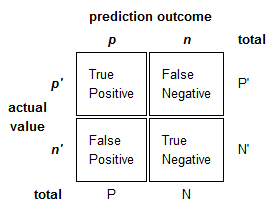
\includegraphics[width=6in]{images/confusionmatrix.png}
	\caption{Confusion Matrix} %figure name
	%\caption*{Source: https://rasbt.github.io/mlxtend/user_guide/evaluate/confusion_matrix/}
	%\0caption*{Source: https://istqbexamcertification.com}
	\label{Confusion matrix} % for referencing
\end{large}
\end{figure} 
\par
Terminology and derivatives from confusion matrix.
\begin{enumerate}
\item \textbf{Accuracy (ACC):}
\par $$ACC = \frac{TP+TN}{P+N} =\frac{TP+TN}{Total}$$

\item \textbf{Error (ERR):}
\par $$ERR = \frac{FP+FN}{P+N} =\frac{FP+FN}{Total}$$


\item \textbf{Sensitivity or True Positive Rate (TPR):}
\par $$TPR = \frac{TP}{P}=\frac{TP}{TP+TN}$$

\item \textbf{False Positive Rate (FPR):}
\par $$fPR = \frac{FP}{N}=\frac{FP}{FP+TN}$$
\item \textbf{Specificity or True Negative Rate(TNR):}
\par $$TNR = \frac{TN}{N}=\frac{TN}{FP+TN•}$$

\item \textbf{Positive Predictive Value(PPV):}
\par $$PPV = \frac{TP}{TP+FP}$$
 
\item \textbf{Negative Positive Value(NPV):}
\par $$NPV = \frac{TN}{TN+FN}$$ 

\item \textbf{Negative Predictive Value(NPV):}
\par $$ACC = \frac{TP+TN}{P+N}$$

\item \textbf{F1 Score:}
\par $$F1=\frac{2TP}{P+P'} $$


\end{enumerate}

\section{Implementing Algorithm}
\begin{itemize}
\item Problem Statement

\begin{itemize}
 \item Given Features : $X_1,X_2,X_3.....X_n.$
 \item Predict a label Y.
\end{itemize}

\item Consider each attribute and class label as random variables.
\item Given a record with attributes ($A_1,A_2,A_3.....A_n)$.
\begin{itemize}
\item Goal is to predict class C.
\item Specifically find value that maximizes P(C$|A_1,A_2,A_3.....A_n)$
\end{itemize}
\item Compute posterior probability P(C$|A_1,A_3,A_3.....A_n)$ for all value of C using Bayes theorem.
\[P(C|B)=\frac{P(A_1*A_2*A_3*.....*A_n|C)P(C)}{P(A_1*A_2*A_3*.....*A_n)}\]
\item Choose value that maximizes P(C$|A_1,A_2,A_3.....A_n)$
\item Equivalent to choosing value of C that maximizes.
$P(A_1,A_2,A_3.....A_n|C)P(C)$

\item Assume independence among attributes $A_i$ when class is given:
\begin{itemize}
\item $P(A_1,A_2,A_3.....A_n|C)P(C)=P(A_1|C_j)P(A_2|C_j)P(A_3|C_j)...P(A_n|C_j)$.
\item Estimate $P(A_i|C_j)$ for all $A_i$ and $C_j$.
\item New point is classified to $C_j$ if
\par 
$P(C_j)*P(A_i|C_j)$ is maximum.
\end{itemize}

\end{itemize}



\chapter{Methodology}
\section{E-R Diagram}
The Entity Relationship Diagram of the project:
\par
\begin{figure}[tbh] % tbh means top, bottom or here (priority: left to right)
\begin{large}

	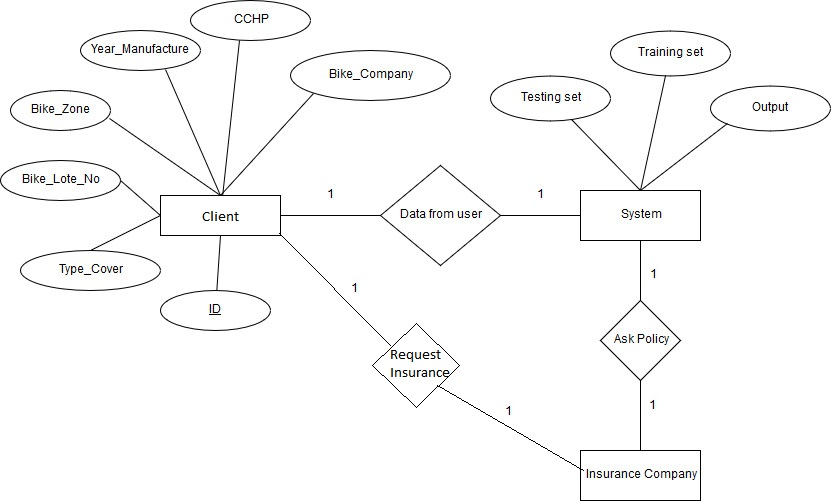
\includegraphics[width=6in]{images/ER.jpg}
	\caption{Entity Relationship Diagram} %figure name
	\label{ER} % for referencing
\end{large}
\end{figure}
\newpage
\section{Flow Chart}
\begin{figure}[tbh] % tbh means top, bottom or here (priority: left to right)
\begin{center}
	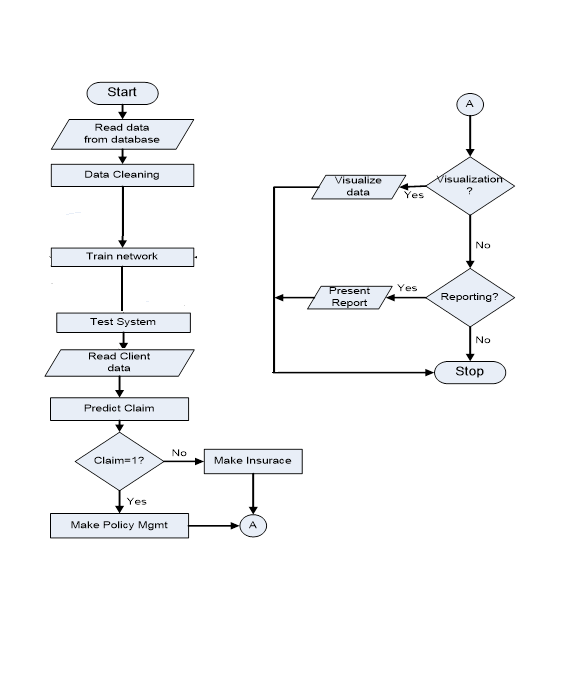
\includegraphics[height=7in]{images/systemflow.png}
	\caption{Flow Chart Of Project} %figure name
	
	\label{Flow Chart} % for referencing
\end{center}
\end{figure}


\pagebreak
\newpage
\section{Use-Case}
\begin{figure}[tbh] % tbh means top, bottom or here (priority: left to right)
\begin{center}
	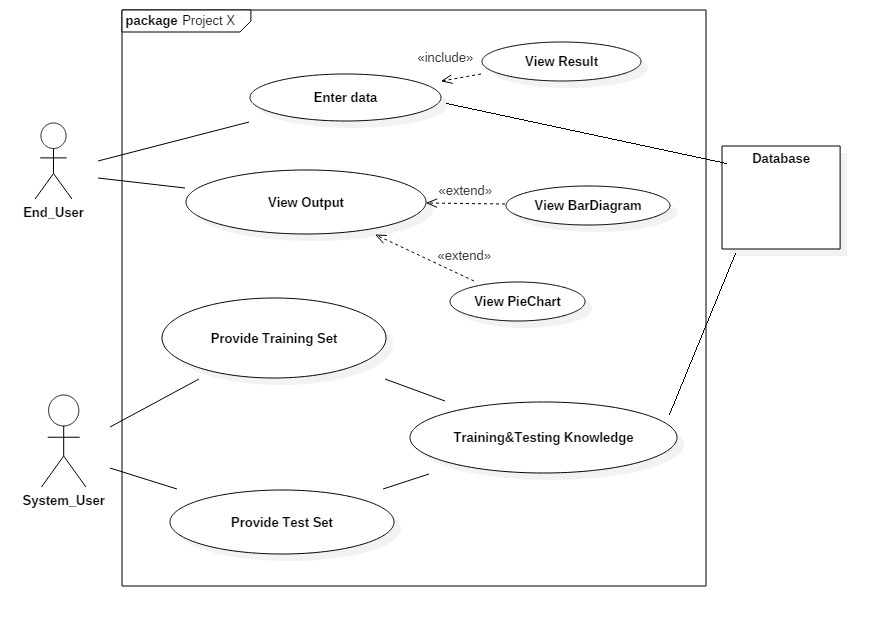
\includegraphics[width = 6in]{images/uc.jpg}
	\caption{Use-case Diagram} %figure name
	\label{Use-case} % for referencing
\end{center}
\end{figure}

In this project there will be three options. The customers information will be taken and based on which insurance to be done is decided. Report and Visualization of data based on various attributes can be done which helps to know the progress of an insurance company.
\newpage
\section{Class  Diagram}
\begin{figure}[tbh] % tbh means top, bottom or here (priority: left to right)
\begin{center}
	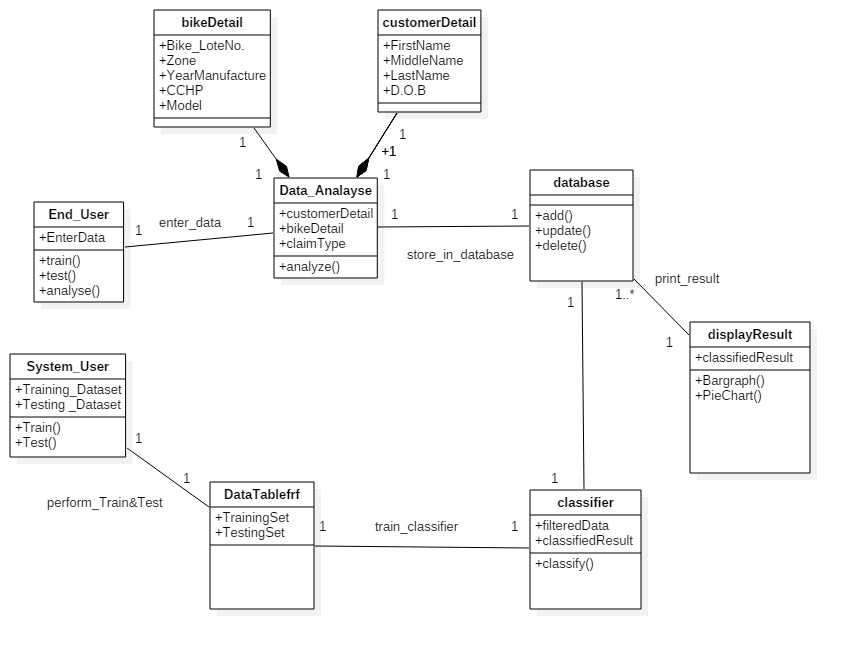
\includegraphics[width = 6in]{images/Cd.png}
	\caption{Class Diagram} %figure name
	\label{Class} % for referencing
\end{center}
\end{figure}


\newpage
\section{Sequence Diagram}
\begin{figure}[H] % tbh means top, bottom or here (priority: left to right)
\begin{center}
	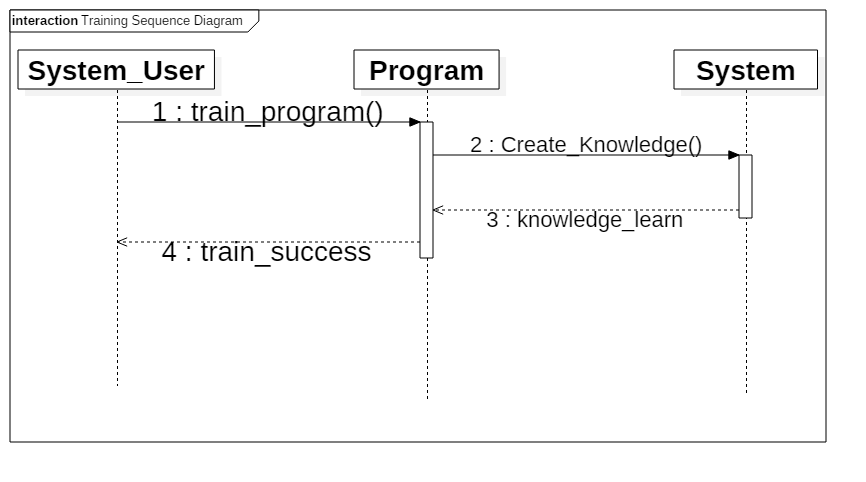
\includegraphics[width = 6in]{images/TrainingSequence.png}
	\caption{Sequence Diagram: Training} %figure name
	\label{Sequence} % for referencing
\end{center}
\end{figure}

%//////////////////\\\\\\\\\\\\\\\\\
\begin{figure}[H] % tbh means top, bottom or here (priority: left to right)
\begin{center}
	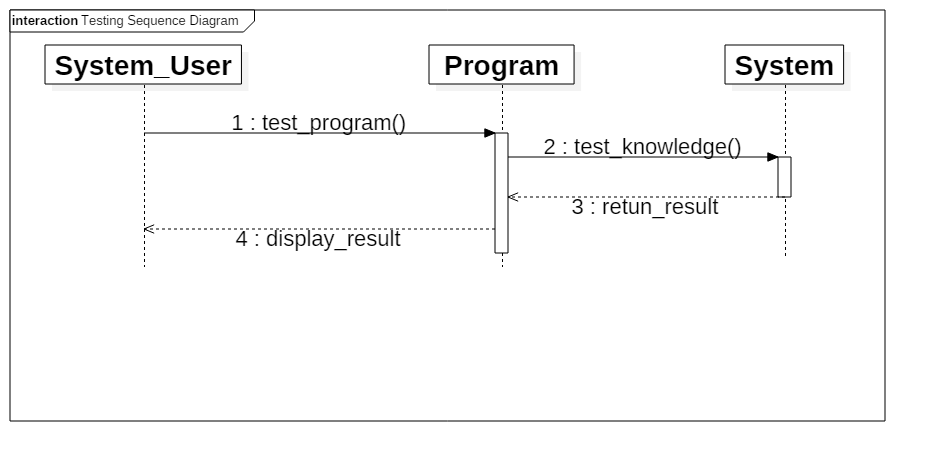
\includegraphics[width = 6in]{images/TestingSequence.png}
	\caption{Sequence Diagram: Testing} %figure name
	\label{Sequence} % for referencing
\end{center}
\end{figure}

\begin{figure}[H] % tbh means top, bottom or here (priority: left to right)
\begin{center}
	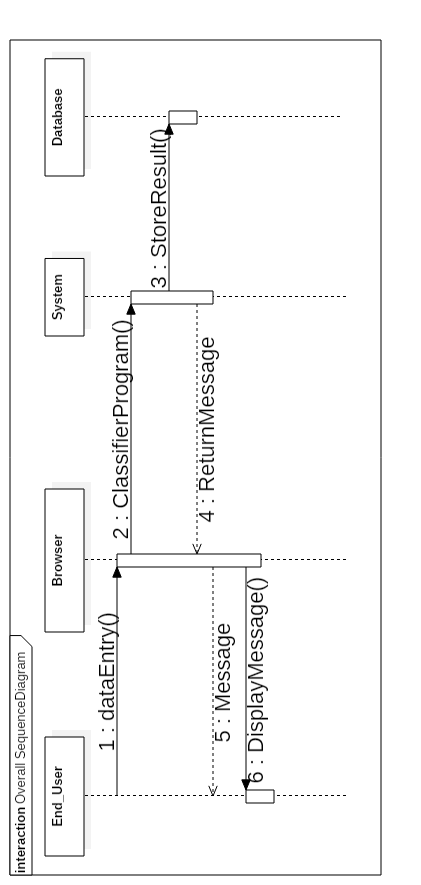
\includegraphics[height = 9in]{images/Sequence.png}
	\caption{Sequence Diagram} %figure name
	\label{Sequence} % for referencing
\end{center}
\end{figure}

\newpage
\section{Collaboration Diagram}

\begin{figure}[H] % tbh means top, bottom or here (priority: left to right)
\begin{center}
	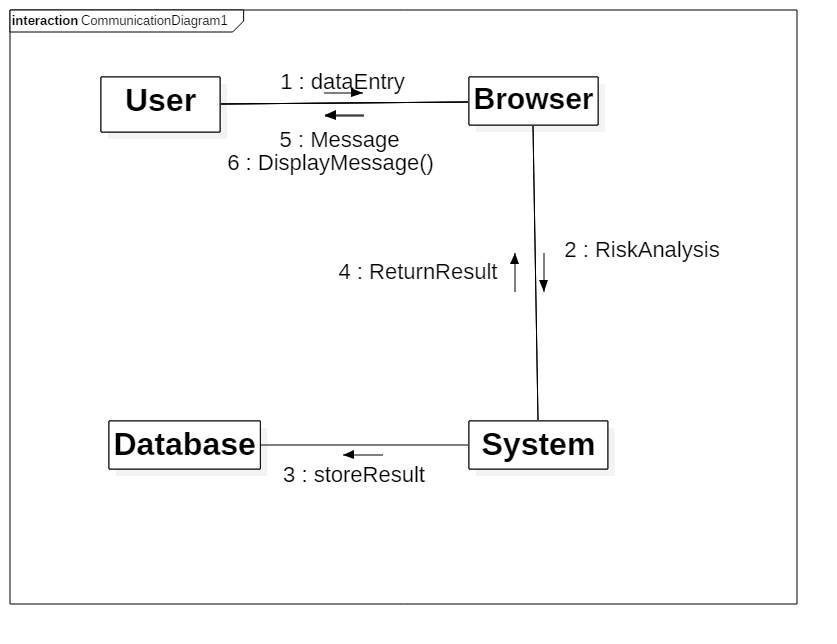
\includegraphics[width = 6in]{images/Collaboration.png}
	\caption{Collaboration Diagram} %figure name
	\label{Collaboration} % for referencing
\end{center}
\end{figure}
\newpage
\section{Software Development Process}
Project-X is prepared by following approaches based on incremental software development model.  The objective of following incremental model, it provides flexibility of starting project by available requirements, such that requirements can be added on the basis of later added projects objectives.  One of the main feature of the model, it
provides designing, testings phase in each increment.

\begin{figure}[tbh] % tbh means top, bottom or here (priority: left to right)
\begin{center}
	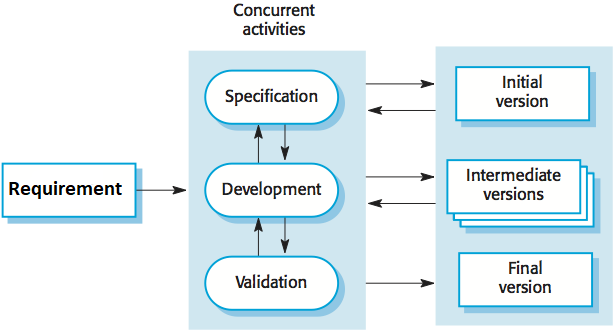
\includegraphics[width = 5in]{images/sdlc.png}
	\caption{Incremental Development Model Chart} %figure name
	\caption*{Source: https://istqbexamcertification.com}
	%/what-is-incremental-model-advantages-disadvantages-and-when-to-use-it}
	\label{Incremental Development Model Chart} % for referencing
\end{center}
\end{figure}
\par 
$  $
Project-X is application based on Na\"{\i}ve Bayesian Classifier for classifier data and predict the result for user.
We mainly divide our project into 3 phase.
\begin{enumerate}
	\item[1.] \textbf{1st Incremental Phase}
	\par
	As Initial phase, we mainly involved in researching about our project basic idea. We also visit company to get data insurance data that is vital for  our project. We have done most of front end. 
	 \item[2.] \textbf{2nd Incremental Phase}
	 \par 
	 We started with implementing of algorithm and training and testing of data was done to find accuracy of data from collected data. We also get more data from company for further analysis of program. At this, point we were able make the system 60\% accurate. The accuracy remain low due to large variation in claimed and unclaimed data.
	 \newpage
	 \item[3.] \textbf{3rd Incremental Phase}
	 \par 
	 We completed all the system designing part. We tested our program with 82\% accuracy and crystal report. We were able to increase the accuracy by almost 20 \% by using the Data smoothing techniques.
 We used SMOTE process to decrease the variation of data of claimed and unclaimed data. We generated the visual result for easy analysis.
 
\end{enumerate}







\chapter{Result and Discussion}
\section{Outputs}
We successfully completed the the Project-X an online platform to check whether to selected or rejected as per data entered. We have used a Na\"{\i}ve Bayesian Classifier for creation of model on the basis  of data we feed to the classifier that will predict the either to claimed or unclaimed the data.
\par
Data have been collected from Nepal Insurance Company, Kamaladi, Kathmandu and we have pre-processed and normalized data such that 5 lakhs data have been reduced to 6xxx. We have extract only six set of data from the bunch, We extract the data of 6 attributes namely Bike Manufacturer,Manufacture year,Bike CC, Bike zone, Bike Lote no and insurance type cover. These data were strings or the range of numeric data. These data are normalized to increase the accuracy and prevent from diverging.
The normalized data are used to built up up the  model. Due to large variation of the claimed and unclaimed data, we use smoothing techniques to maintain the ratio.

\par
Using confusion matrix we have obtained 82\% accuracy. Using the same pre-processed and normalized data we have prepared report that can be printed and provided to individual member of management using Crystal Reporting and visualize through bar chart using feature of Visual Studio such that it depicts overall performance of the insurance of bike based on selected attributes.



\section{Limitation}
Using Na\"{\i}ve Bayesian Classifier, we created the model based upon the data of bike provided by company. Even though we have created a full working system it have some limitations.
\begin{enumerate}
\item Limited to the Bike Insurance only.
\item Data Based on single company only.
\item use of existing data only.
\end{enumerate}


 
\section{Problems Faced}
\begin{itemize}
\item Data filtering through various process. 
\item Limited no of claimed data.
\item Implementing the Algorithm.
\item Generating report.
\end{itemize}

\section{Work Schedule}
\begin{figure}[tbh] % tbh means top, bottom or here (priority: left to right)
\begin{center}
	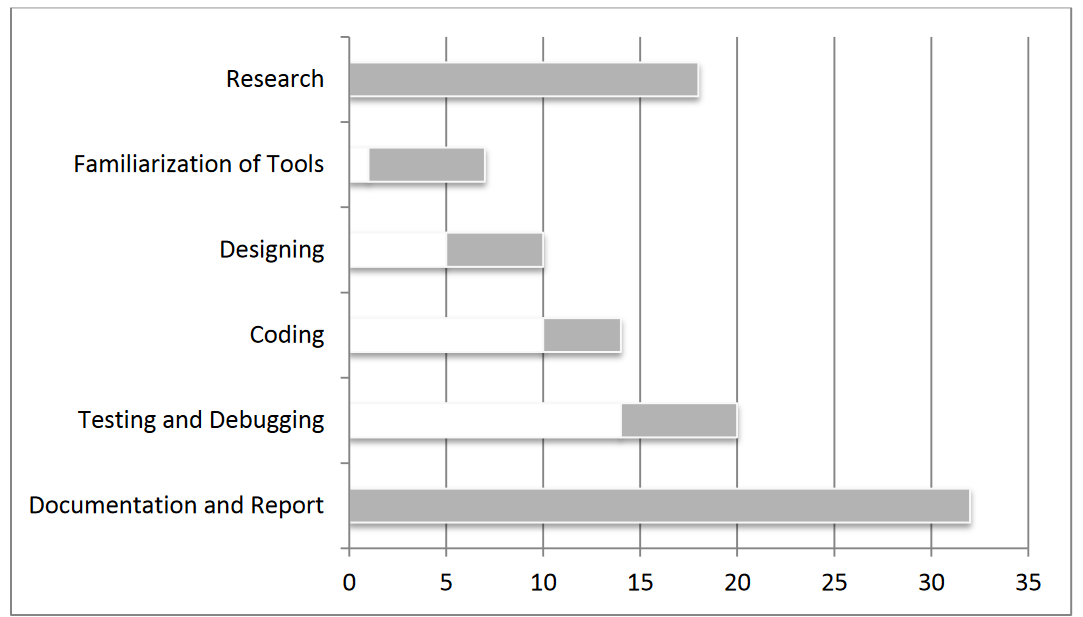
\includegraphics[width=5in]{images/gantt.png}
	\caption{Gantt Chart} %figure name
	\label{Gantt chart} % for referencing
\end{center}
\end{figure}


\section{Future Enhancement}
\begin{enumerate}
\item Increase domain to accommodate  all automobiles 
\item Collects data from many insurance company as far as possible
\item Connecting the system with the company server and update data simultaneously
\end{enumerate}


\renewcommand\bibname{References} % Change heading to References
\bibliographystyle{IEEEtran} % to use IEEE Format for referencing
\addcontentsline{toc}{chapter}{References} % to add references in TOC
\bibliography{ref} % specify the .bib file containing reference information 


\end{document}

